\chapter{Introducción}
\label{introduccion}

La introducción responde cinco preguntas:
\begin{description}
\item[¿en que tema están trabajando? ] Introduce en contexto en el que están trabajando (p.e., el ámbito en el que se dá el problema). Da definiciones (brevemente) de conceptos que aparecen en el contexto. 
\item[¿cual es el problema? ¿es interesante? ] Presenta el problema que se quiso resolver (o la necesidad que se quiso cubrir), y explica por que es relevante y no es trivial resolverlo.  Introduce definiciones (brevemente) que ayuden a entender el problema. Esta parte (en conjunto con la anterior) dan la motivación del trabajo. 
\item[¿cual es la estrategia general de solución? ] Presenta en términos generales la estrategia de solución (p.e., cuenta que se desarrolló un sistema que permite... y que por su característica... resuelve el problema planteado.
\item[¿cuales son las contribuciones del trabajo? ] Enumera que es lo que obtiene quien lee el trabajo. Ejemplos de contribuciones son: un análisis detallado del problema X en el contexto Y, una comparación de tecnologías de servidores ZZZ, una revisión de literatura del estado actual del tema J, una arquitectura y diseño de un sistema que permite..., un prototipo que muestra como la arquitectura Z puede implementarse de forma B, evidencia experimental que muestra que es posible WW, un framework/libreria web para GGG, un algoritmo eficiente para ...   
\item[¿Cómo esta organizado el trabajo?] El ultimo párrafo de la Introducción explica como esta organizado el documento; como se lee, que es lo que se va a encontrar en cada capítulo y como se relacionan.   
\end{description}

Dependiendo de lo larga que quede puede tener varias secciones. No estaría mal que esas secciones se llamen ``Motivación''\footnote{prestá atención a como se ponen las comillas en LaTex} (que habla del contexto y el problema), ``Enfoque'' (que explica como lo van a hacer), ``Contribuciones'' y ``Organización''.  

Muchos dicen que la intro se puede escribir al final. De hecho, las contribuciones y la organización es algo que está claro solo al terminar el proyecto de tesis. Sin embargo, creo que tener un borrador corto de la intro (un párrafo respondiendo a cada una de las preguntas) es bueno para utilizarlo como referencia cada vez que nos olvidamos que es lo que queríamos hacer. 


\section{Algunas palabras sobre este documento}

Mi idea al escribir este documento es que sirva como punto de partida para organizar la tesis (el proyecto y el documento) y como punto de partida para editar el documento en LaTex. Hay muchas referencias en la web con guías similares. Todas tienen algo bueno. La página web de Willilam Shoaff Shoaff \cite{Shoaff} habla sobre como organizar una tesis de maestría (lo cual creo que es aplicable a la tesis de Licenciatura). Si se imaginan un futuro escribiendo artículos técnicos y están con tiempo para leer, les recomiendo el libro de Justin Zobel "Writing for Computers Science" \cite{Zobel04a} que está en biblioteca de Informática de UNLP. En la Figura \ref{zobel-page-46} se pude ver un extracto de libro en el que discute el poco valor que tienen palabras como "muy" en la escritura técnica. 

\begin{figure}
\begin{center}
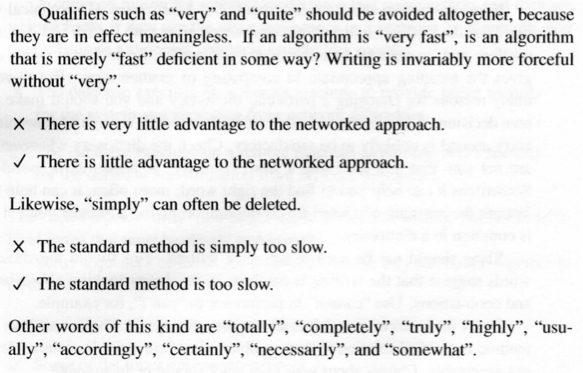
\includegraphics[width=0.8\textwidth]{00-introduccion/zobel-page-46}
\caption{Extracto del libro Writing for Computers Science de Justin Zobel}
\label{zobel-page-46}
\end{center}
\end{figure}

